\chapter{Nowa metoda oceny procesu gojenia ścięgna Achillesa}
\label{NewMethod}

%ATRS \cite{Kearney2012}, VISA-A \cite{Robinson2001} or FAOS \cite{Roos2001} - dorzuć do biomechaniki.

%	Medical Imaging - especially Magnetic Resonance Imaging (MRI) and Ultrasonography (US) - is one of the most common technique that nowadays is used to monitor soft tissues. Some papers e.g.  \cite{Khan2003, Ibrahim2013} indicate the advantage of MRI over US showing that MRI appearance can be easier associated with the clinical outcomes. Despite this, US also present in e.g. \cite{vanSchie2009, PradoCosta2018} as a valuable technique for the soft tissues properties investigation, yet technical issues and lack of standardization limits its use.} - dorzuć do USG/MRI

W tym rozdziale zostanie zaprezentowana autorska propozycja metody oceny procesu gojenia się ścięgna Achillesa bazująca na badaniach obrazowych. W szczególności przedstawiony zostanie ilościowy opis, umożliwiający w zobiektywizowany sposób ocenę morfologii tkanek widocznych w obrazach Rezonansu Magnetycznego i Ultrasonografii. Finalnie zostanie również zaproponowane nowatorskie podejście do automatycznego wyliczania wskazanych w opisie procesu parametrów, co jest najważniejszym osiągnięciem całości tej pracy. 

Wskazana automatyzacja została przez autora wykonana dla danych z Rezonansu Magnetycznego, które zostały przez specjalistów wskazane jako klinicznie bardziej istotne niż USG. Niemniej jednak dane Ultrasonografii zostały również przeanalizowane pod kątem wartości dodanej do całego proponowanego procesu.  

W chwili pisania tej pracy nie istnieje wedle najlepszej wiedzy autora podejście umożliwiające zobiektywizowany i co ważniejsze automatyczny sposób oceny badań obrazowych prezentujących gojące się ścięgno Achillesa. Stąd implikacje dotyczące trudności z integracją subiektywnych interpretacji ze skalami testów funkcjonalnych takich jak ATRS i w rezultacie zmniejszona efektywność całego procesu oceny rehabilitacji. 

Podczas próby rozwiązania wskazanego problemu autor tej pracy w szczególności chce skupić się na dwóch aspektach. Pierwszym z nich jest jakość generowanej automatycznie oceny odniesiony do jakości wzorca tj. oceny doświadczonego radiologa. Drugim natomiast jest czas akwizycji danych, a zatem wybór praktycznego protokołu, który zapewni możliwie krótki udział pacjenta w badaniu. W obu przypadkach celem jest poszukiwanie punktu optimum, w którym maksymalizowana będzie jakość oceny, a minimalizowany czas, zarówno radiologa jak i pacjenta, niezbędny do wykonania koniecznych czynności. Szczegóły podejścia zostały opisane w kolejnej sekcji.

   

%\textcolor{blue}{The perturbations in the healing process of the Achilles tendon may result from the surgery, further rehabilitation and other factors like diet, obedience to treatment guidelines and patient predispositions. Thus, challenges in the assessment process are connected to the proper recognition of the morphological changes of the tendon structure, its functional limitations, and individual features.}

%\textcolor{blue}{


%\textcolor{blue}{Particularly there is no structured description that could apply to MRI and US studies of the Achilles tendon. The existing approaches like ATRS  \cite{Kearney2012}, VISA-A \cite{Robinson2001} or FAOS \cite{Roos2001} are only suitable for measuring the general outcome, related to symptoms and physical activity of patients. The motivation for our work is to utilize medical imaging techniques to improve precise monitoring and comparison of different therapies for ruptured Achilles tendon.}

%\textcolor{blue}{Thus we performed a broad study on 60 patients who underwent the open surgical reconstruction. The patients were monitored over a year of rehabilitation with the use of 10 MRI and 2 US protocols, acquired in 10 properly distributed time-steps. We also gathered a homogeneous control group composed of 29 healthy volunteers. To our best knowledge, there is no such study comparable in scale to the one that we introduce in this paper. For example, in\cite{Tam2017} the conclusions are formulated based on two samples, in \cite{Fujikawa2007} the authors evaluate a total of 30 healing tendons repaired with a percutaneous surgical technique and 10 repaired with an open surgical one, finally in \cite{Albano2017} the authors present results for 43 patients to study the significance of growth factors.}


\section{Metodyka}

W tej sekcji zostanie szczegółowo opisana proponowana metoda automatycznej oceny procesu gojenia się ścięgna Achillesa widocznego w badaniach obrazowych Rezonansu Magnetycznego. Dodatkowo scharakteryzowany zostanie zbiór danych, który posłużył do opracowania rozwiązania, jak również ankieta walidacyjna stanowiąca wzorzec odniesienia dla przedstawionej metody. 

Autor tej pracy, w proponowanym podejściu skorzystał z metod widzenia komputowego, a dokładniej z fuzji algorytmów sztucznej inteligencji i przetwarzania obrazów. W kontekście tej pracy, pierwsze znajdują swoje zastosowanie do ekstrakcji wektora cech dla danej reprezentacji obrazowej. Drugie, pozwalają uwzględnić wiedzę dziedzinową w procesie numerycznej oceny.

W przypadku algorytmów sztucznej inteligencji zastosowano  opisane w Rozdziale \ref{CNNs} konwolucyjne sieci neuronowe, a dokładniej AlexNet, GoogLeNet (inceptionV3) i ResNet-18. W pierwszej kolejności wykonane zostało szkolenie podanych sieci dla problemu binarnej klasyfikacji tj. odróżniania obrazów chorego od zdrowego ścięgna. Następnie część klasyfikująca została usunięta z topologii sieci, pozostawiając ekstraktor cech z parametrami zoptymalizowanymi pod kątem wydobycia istotnej informacji opisującej różnice między zdrową i chorą tkanką. Na tak otrzymanym wektorze, przeprowadzono redukcję wymiarowości z wykorzystaniem metody PCA (zob. \ref{DimReduction}). W wyniku przeprowadzonych eksperymentów, ostatecznie zdecydowano się uwzględnić 200 pierwszych czynników głównych w końcowym rozwiązaniu.

W przypadku metod przetwarzania obrazów zastosowano obliczenia cech z wydzielonego przez specjalistę radiologa ROI (od ang. \textit{Region of Interest}) reprezentującego tkanki otoczone ościęgnem. Sumarycznie wyliczono 46 klasycznych cech obrazowych, w tym pole powierzchni ROI, 9 cech opisujących statystykę wartości pikseli i 36 cechy Haralick'a opisujące teksturę (zob. \cite{Haralick1973}). W ramach statystyk scharakteryzowano: min, max, średnią, odchylenie standardowe, skośność, kurtozę, 25-percentyl, medianę oraz 75-percentyl. Natomiast w ramach cech Haralick'a: drugi moment kątowy, kontrast, korelacja, wariancja, odwrotny moment różnicowy, suma średnich, suma wariancji, suma entropii, entropia, różnica wariancji i maksimum prawdopodobieństwa. Cechy Haralick'a wyliczono dla 3 dystansów separacji \textit{d}=1,5,10. Dokładna metoda selekcji powyższych cech została przedstawiona w pracy  \cite{Nowosielski17}.  

Spośród tak wyliczonych 246 cech dokonano selekcji metodą LASSO (zob. [opis]). W rezultacie dla wszystkich ocenianych parametrów uzyskano optymalną mieszaninę poniżej 20 cech ekstrahowanych z wykorzystaniem sieci konwolucyjnych oraz klasycznych metod obrazowych. Wybrane predyktory posłużyły do szkolenia algorytmu meta-regresji, przy użyciu którego wykonana została fuzja.   

Końcowa ocena badania została wykonana następującą metryką $H$ zaproponowaną przez autora tej pracy:
\begin{equation}
H = TM(R(x_1), R(x_2),..., R(x_n))
\end{equation}
gdzie $TM$ jest średnią trymowaną z marginesami 2.5\%, a $R(x_i)$ jest wynikiem regresji obliczonym dla przekroju osiowego $x_i$, gdzie $i$ to indeks przekroju w trójwymiarowym badaniu RM.

Schemat powyższej metody został zaprezentowany na Fig. \ref{fig:net}. 
\begin{figure}[h!]
	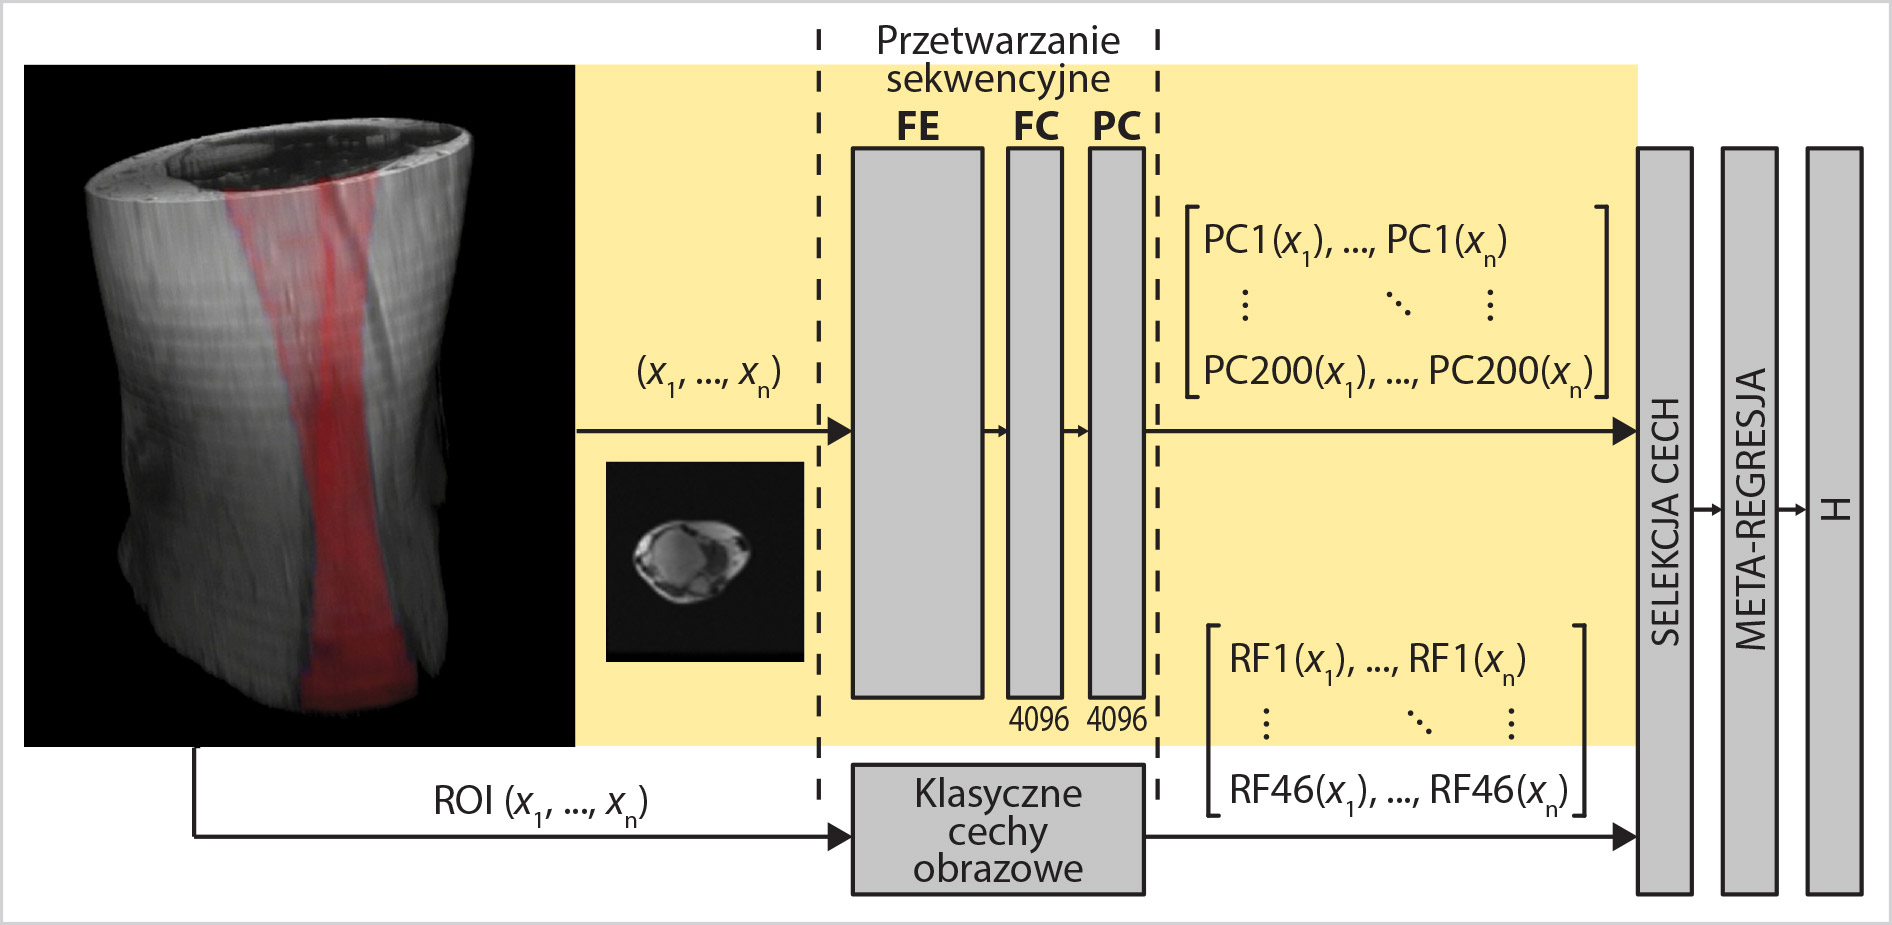
\includegraphics[width=\textwidth]{figures/net.jpg}
	\caption{Schemat automatycznej metody oceny procesu gojenia się ścięgna Achillesa.} \label{fig:net}
\end{figure}
W ogólnym ujęciu trójwymiarowe badanie RM dzielone jest na pojedyncze przekroje osiowe, które stanowią dane wejściowe do oznaczonej na żółto części opartej o metody głębokiego uczenia się. Początkowo dane przetwarzane są prze ekstraktor cech sieci AlexNet wybranej w wyniku eksperymentów (FE). Następnie wstępnie grupowane są z wykorzystaniem warstwy fully connected (FC) i poddane redukcji z 4096 pojedynczych wyjść aktywacyjnych do 200 czynników głównych (PC).

Równolegle, ROI z każdego z przekrojów stanowi dane wejściowe do części obliczeń klasycznych cech obrazowych. Końcowa fuzja wyselekcjonowanych cech z wykorzystaniem meta-regresji i metryki $H$ zapewnia numeryczny opis składający się z pojedynczej wartości dla całego badania RM w każdym z ocenianych parametrów.

\subsection{zbiór danych}

Dane wykorzystane w tej pracy zostały zebrane w ramach projektu START "Wykorzystanie autologicznych mezenchymalnych komórek macierzystych w procesie regeneracji rekonstruowanego ścięgna Achillesa" finansowanego z konkursu STRATEGMED1 prze Narodowe Centrum Badań i Rozowoju. W ramach projektu do badanej grupy zakwalifikowano 60 pacjentów po całkowitym zerwaniu ścięgna Achillesa i 29 ochotników stanowiących grupę odniesienia. 

Kryteria wykluczające z grupy badanej zostały zdefiniowane tak aby kwalifikowani pacjenci nie posiadali wcześniejszej historii urazów ścięgna Achillesa ani przewlekłych chorób, które mogłyby spowodować degenerację tkanki ścięgnistej. Uwzględniono również warunki odbiegające od normy takie jak: otyłość ciąża, infekcje. Ostatecznie, w ramach grupy pacjentów znalazło się 49 mężczyzn i 11 kobiet w wieku pomiędzy 24 a 49 lat i ze średnią wieku 36 lat. Wszyscy pacjenci podpisali stosowne zgody wymagane do przeprowadzenia badań.   

52 z pośród 60 pacjentów zerwało ścięgna podczas uprawiania sportu. Dokładniej były to: piłka nożna (19), squash/tenis (8), koszykówka (4), bieganie (3), podskoki (2), siatkówka (2) oraz badminton, box, piłka ręczna, fitness, cross-fit, skateboard, rugby i skakanka. Urazy w 31 przypadkach dotyczyły prawego ścięgna, a w 29 lewego. Średnia pozycja zerwania umiejscowiona była 57.11 mm ponad górnym konturem kości piętowej.

W okresie do tygodnia po urazie pacjenci przeszli zabieg rekonstrukcji wykonany metodą szycia na otwartym ścięgnie (zob. \ref{gojenie}). Następnie rozpoczęto rehabilitacje trwającą 12 miesięcy monitorowaną z wykorzystaniem Rezonansu Magnetycznego, Ultrasonografii. Wykonano również badania biomechaniczne na początku i na końcu okresu rehabilitacji zgodnie zgodnie z protokołem opisanym w sekcji \ref{biomechanika}.

\subsubsection{Rezonans magnetyczny:}
Przy akwizycji danych z wykorzystaniem RM posłużono się aparatem GE Signa HDxt 1.5T wyposażonym w cewkę Foot \& Ankle dedykowaną do pomiarów w rejonie dolnej kończyny. Każde z badań RM było wykonane z użyciem 7 sekwencji i łącznie 10 modalności opisanych szczegółowo w sekcji \ref{RM} tj.:
\begin{enumerate}
	\item T1 zależne
	\item T2 zależne
	\item PD
	\item T2 mapping
	\item T2 $^\ast$ GRE
	\item T2 $^\ast$ GRE TE\_MIN
	\item 3D FSPGR
	\begin{itemize}
		\item In Phase Ideal
		\item Out Phase Ideal
		\item Fat Ideal
		\item Water Ideal 
	\end{itemize}
\end{enumerate}

Z wykorzystaniem powyższych sekwencji na grupie zdrowych ochotników przeprowadzono pojedyncze badanie, natomiast pacjentów skanowano 10-krotnie w odpowiednio zdefiniowanych odstępach czasowych. Pierwsze badanie odbyło się przed operacją, a następnych 9 po, odpowiednio w: 1, 3, 6, 9, 12, 20, 26, 40 i 52 tygodniu. W procesie zbierania danych wystąpiły problemy wynikające z braku obecności poszczególnych osób na badaniach lub niespójnością danych. Dlatego finalnie skompletowany zbiór składa się z homogenicznych badań 27 zdrowych ochotników (270 trójwymiarowych skanów RM, w skład których wchodzi wspomniane 10 modalności) oraz badań 59 pacjentów (5900 trójwymiarowych skanów RM, w skład których wchodzi 10 modalności i 10 kroków czasowych). Przykładowe wizualizacja danych pacjenta i osoby zdrowej znajduje na Fig. \ref{fig:MRI_sample}. 
\begin{figure}[h!]
	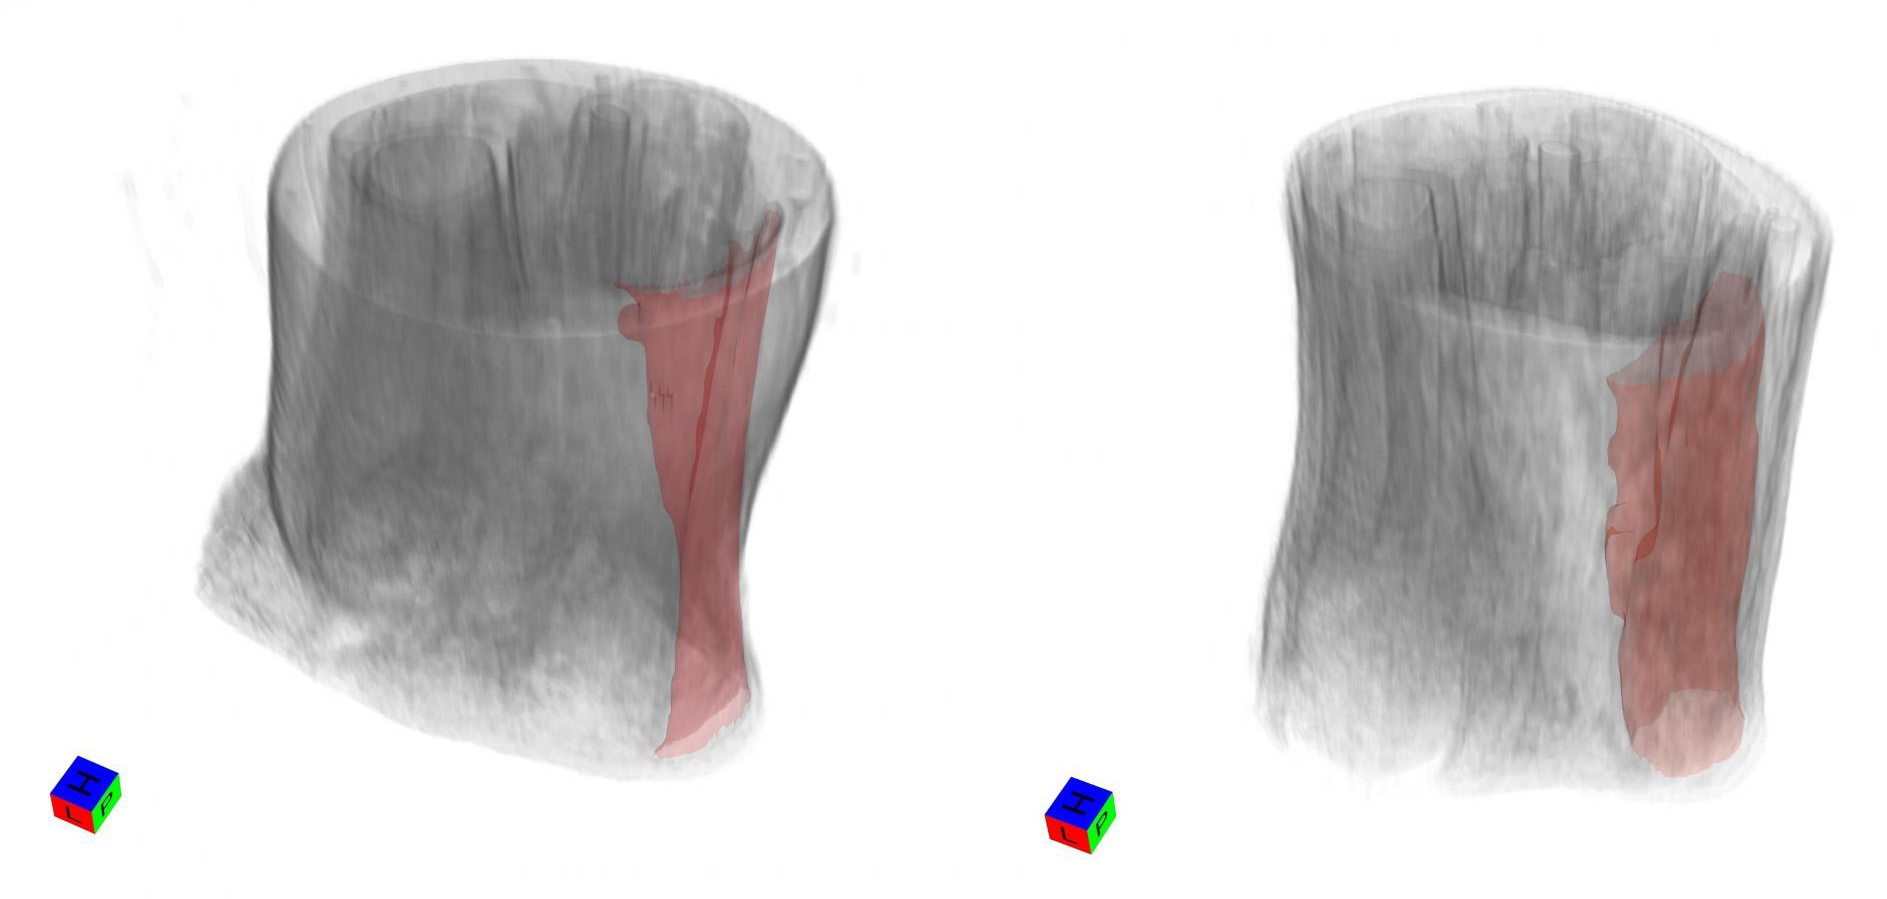
\includegraphics[width=\textwidth]{figures/Data_MRI_sample.png}
	\caption{Wizualizacja przykładowych danych RM w sekwencji PD dla zdrowego (po lewej) i gojącego się (po prawej) ścięgna Achillesa.}
	 \label{fig:MRI_sample}
\end{figure}
Obszar zajmowany przez tkankę ścięgnistą został oznaczony na czerwono. Należy zwrócić uwagę na różnicę w kształcie, która dla zdrowego przykładu jest zgodna z opisem anatomicznym ujętym w sekcji \ref{anatomia} natomiast dla przykładu chorego zawiera liczne deformacje.

Powyższe zbiory trójwymiarowe posłużyły do opracowania zbiorów dwuwymiarowych zawierających przekroje. W ten sposób udało się zwiększyć liczbę próbek wejściowych potrzebnych do szkolenia sieci neuronowych. Dane RM charakteryzują się wysoką anizotropią i ich rozdzielczość wynosi przykładowo 512$\times$512$\times$Z, gdzie $Z\in(10:50)$ (wyjątkiem jest sekwencja 3D FSPGR charakteryzująca się niższą anizotropią, jednak większą ilością artefaktów wynikających z szybkiego czasu akwizycji). Dlatego zbiory oparte o RM zostały stworzone w oparciu o przekroje osiowe 512$\times$512. W zależności od eksperymentów służących do doboru parametrów i komponentów metody wykorzystano:
\begin{itemize}
	\item powiększony zbiór treningowy RM -- zawiera przekroje osiowe ze wszystkich badań (z wyłączeniem pacjentów testowych) realizowanych wszystkimi sekwencjami. Dodatkowo liczba przekroi została powiększona poprzez zastosowanie transformacji odbicia lustrzanego i w przypadku chorych przykładów 10 obrotów w zakresie od -10 do 10 stopni. Finalnie zbiór zawiera 234.502 przekrojów oznaczonych jako zdrowych i 277.208 oznaczonych jako chorych.
	\item ograniczony zbiór treningowy RM -- zawiera przekroje osiowe ze zbioru oznaczonych 44 pacjentów jedynie w sekwencji T2 $^\ast$ GRE TE\_MIN (18.863 próbek).
	\item zbiór testowy - zawiera przekroje pochodzące z danych zebranych dla 4 testowych pacjentów.
\end{itemize}

\subsubsection{Ultrasonografia:}
W przypadku danych Ultrasonografii stosowano się do identycznych odstępów czasowych, co w przypadku badań RM i akwizycji poddano tych samych pacjentów. Z przyczyn praktycznych zmniejszyła się jedynie grupa odniesienia, która w tym przypadku wyniosła 18-stu zdrowych ochotników. Badania zrealizowano z wykorzystaniem aparatu GE 3D high-resolution Voluson E8 Expert z liniową sondą (5--18 MHz). Jako dane wejściowe wykorzystano informacje z trybu B (zob. \ref{USG}), których ostateczna liczba wyniosła 565 3D skanów. 

Dane USG są zbliżone do izotropowych dlatego utworzono zbiory zarówno w oparciu o przekroje w płaszczyźnie osiowej jak i strzałkowej:
 \begin{itemize}
 	\item zbiór treningowy USG (strzałkowy) -- zawiera 253.639 2D przekrojów w płaszczyźnie strzałkowej, w tym 245.366 pochodzących od chorych 44 pacjentów oznaczonych przez radiologa i 8.273 pochodzących od zdrowych ochotników.
 	\item zbiór treningowy USG (osiowy) -- zawiera 467.548 2D przekrojów w płaszczyźnie osiowej, w tym 450.816 pochodzących od chorych 44 pacjentów oznaczonych przez radiologa i 16.732 pochodzących od zdrowych ochotników. 
 \end{itemize}

Wizualizacja przykładowych danych USG znajduje się na Rys. \ref{fig:US_sample}
\begin{figure}[h!]
	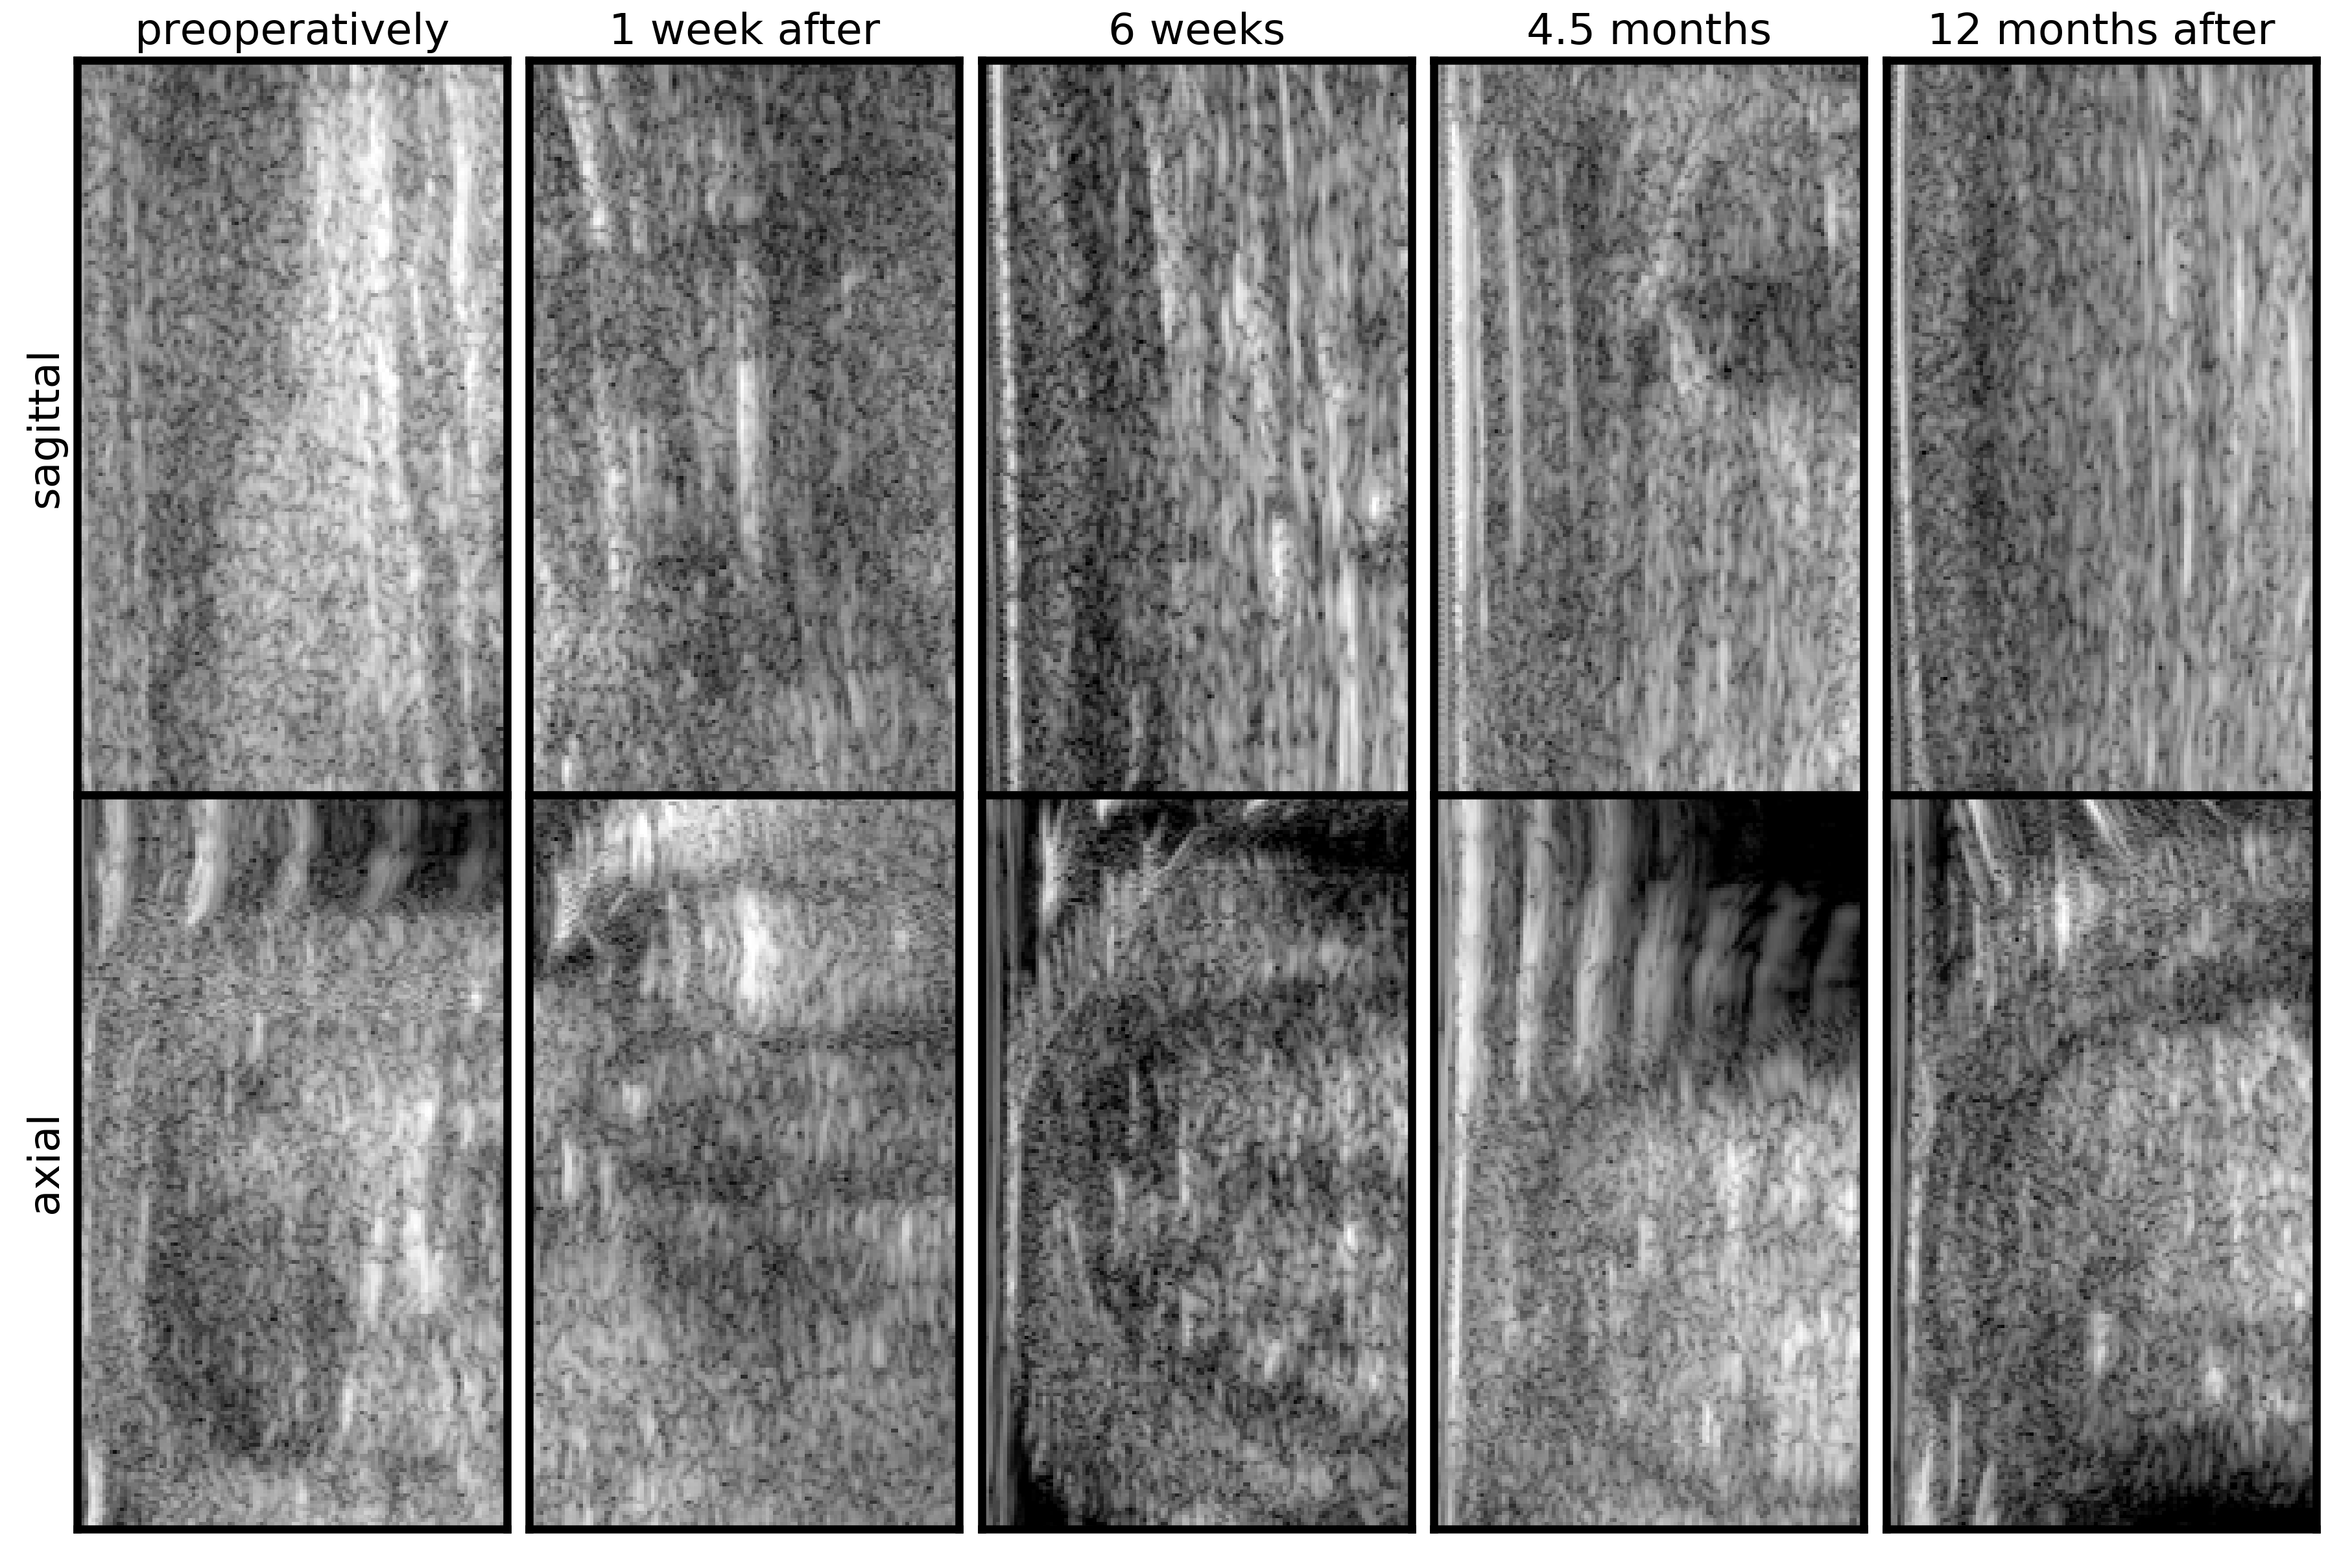
\includegraphics[width=\textwidth]{figures/Data_US_sample.png}
	\caption{Wizualizacja przykładowych danych USG w kolejnych tygodniach po zszyciu ścięgna w przekrojach osiowych i strzałkowych.}
	\label{fig:US_sample}
\end{figure}

Szczegółowa analiza załączonych obrazów może być wykonana jedynie przez specjalistę radiologa, jednak w ogólności można zaobserwować ułożenie włókien ścięgnistych na przekrojach strzałkowych i teksturę oraz tkanki otaczające ścięgno na przekrojach osiowych.
 

\subsection{wzorzec odniesienia}

Do stworzenia wzorca odniesienia, w ramach projektu START, została powołana specjalna grupa robocza składająca się z eksperta radiologa, specjalistów ortopedów i ekspertów od komputerowo wspomaganej diagnostyki. Celem grupy było opracowanie ilościowego opisu, który odzwierciedla elementy, na podstawie których radiolog podejmuje subiektywną opinię. W wyniku prac stworzono zestaw sześciu parametrów oceniany w skali 0--7 opisujący proces gojenia się ścięgna Achillesa widoczny w obrazach RM i Ultrasonografii:

\begin{enumerate}
	\item Uszkodzenia śródścięgniste (SCT od ang. \textit{Structural changes within the tendon}) -- informuje o spójności włókien w obszarze ścięgna. Zawiera się w ROI. Ocena wykonywana zarówno w płaszczyznie osiowej jak i strzałkowej. 0 – całkowity brak uszkodzeń, 1 – bardzo małe uszkodzenia. 2 – małe uszkodzenia, 3 – uszkodzenia średniej wielkości , 4 – dość duże uszkodzenia. 5 – duże uszkodzenia, 6 - bardzo duże uszkodzenia, 7 - ekstremalnie duże uszkodzenia.
	\item Pogróbienie ściegna (TT od ang. \textit{Tendon thickening} -- najgrubsze miejsce w kierunku strzałkowym na widoczne na przekroju osiowym. Zawiera się w ROI. 0 – całkowity brak pogrubienia (3mm-5mm), 1 – bardzo małe pogrubienie - 6mm, 2 – małe pogrubienie - 9mm, 3 – średnie pogrubienie- 12mm, 4 –  dość duże pogrubienie -15mm, 5 duże pogrubienie - 18mm, 6 – bardzo duże pogrubienie - 21mm, 7 – ekstremalnie duże pogrubienie – 24mm.
	\item Ostrość granic ścięgna/rozgraniczenie (STE od ang. \textit{Sharpness of the tendon edges})-- informuje o jakości granicy między tkankami ścięgnistymi i otoczeniem, w szczególności, czy brzeg jest fraktalny. Oceniane na zewnątrz ścięgna w płaszczyznie osiowej. 0 – bardzo duża (idelana) ostrość, 1 – duża ostrość, 2 – dość duża ostrość, 3 – średnia ostrość, 4 – mała ostrość, 5 – bardzo mała ostrość, 6 – minimalna ostrość, 7 – całkowicie nieostre.
	\item Obrzęk ścięgna (TE od ang\textit{Tendon edema}) -- informuje o anomaliach w gromadzeniu się płynów w obszarze ścięgna. Zawiera się w ROI i jest oceniany na przekrojach osiowych. 0 – całkowity brak obrzęku, 1 – bardzo mały obrzęk, 2 – mały obrzęk, 3 – obrzęk średniej wielkości, 4 – dość duży obrzęk, 5 – duży obrzęk. 6 – bardzo duży obrzęk, 7 - ekstremalnie duży obrzęk.
	\item Jednorodność ścięgna (TU od ang. textit{Tendon uniformity}) -- informuje o prawidłowej teksturze poszczególnych przekrojów osiowych jak i podobieństwu sąsiednich, mierzonym w płaszyznie strzałkowej. Zawiera się w ROI. 0 – całkowity brak niejednorodności (jednorodne), 1 – bardzo małe niejednorodności, 2 – małe niejednorodności, 3 – niejednorodności średniej wielkości, 4 – dość duże niejednorodności, 5 – duże niejednorodności, 6 – bardzo duże niejednorodności, 7 –  ekstremalnie duże niejednorodności. 
	\item Obrzęk tkanek (TisE od ang. \textit{Tissue edema}) -- informuje o powiększonym przedziale powięziowym ścięgna. 0  – całkowity brak obrzęku, 1 – bardzo mały obrzęk, 2 – mały obrzęk, 3 – obrzęk średniej wielkości, 4 – dość duży obrzęk, 5 – duży obrzęk. 6 – bardzo duży obrzęk, 7 - ekstremalnie duży obrzęk.
\end{enumerate}

Obrazowania 3D zostały opisane przez eksperta radiologa przy użyciu ankiety zawierającej powyższe parametry. W ramach projektu START udało się zgromadzić opisy dla badań RM i USG 48 pacjentów (480 badań). 4 z nich zostało losowo wydzielonych na początku eksperymentów jako pacjenci testowi. Szczegółowy opis eksperymentów znajduje się w kolejnej sekcji.

\section{Eksperymenty}
\subsection{Rozróżnienie ścięgna zdrowego i po zerwaniu}
\subsection{Obliczanie krzywych gojenia}
\begin{equation}
H = \alpha + \sum_{i=1}^{3}\beta_{i}X_{i} + \sum_{i=1}^{3}\gamma_{i}X_{i}^{2} +
\sum_{\substack{i, j = 1\\ i < j}}^{3}\lambda_{i,j}X_{i}X_{j}
\end{equation}

gdzie $X_i = TM(PC_n(x_1), PC_n(x_2),..., PC_n(x_n))_{i}$ to kolejne predyktory, $TM$ to średnia trymowana z marginesami 2.5\%, $PC_n(x_k)$ to $n$-ty czynnik główny otrzymany przy wnioskowaniu sieci dla przekroju osiowego $x_k$, gdzie $k$ jest indeksem przekroju danego protokołu w trójwymiarowym badaniu RM.

%\subsection{Topologia sieci}
%\subsection{Redukcja wymiarowości}
%\subsection{Miara wygojenia}
